\section{Sequentielle Systeme}

 \begin{multicols}{2}
	\subsection{Taktsignal}
			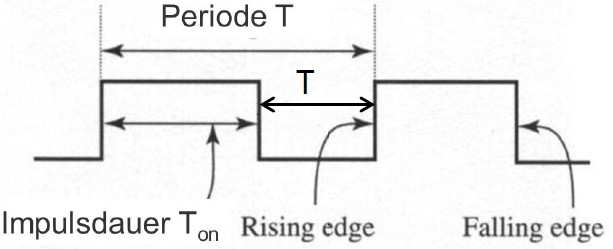
\includegraphics[width=0.6\columnwidth]{pics/taktsignal}
			\newline
			$\mathbf{f=\frac{1}{T}}$ [Hz]
			\columnbreak
		\subsection{l"angster Pfad}
			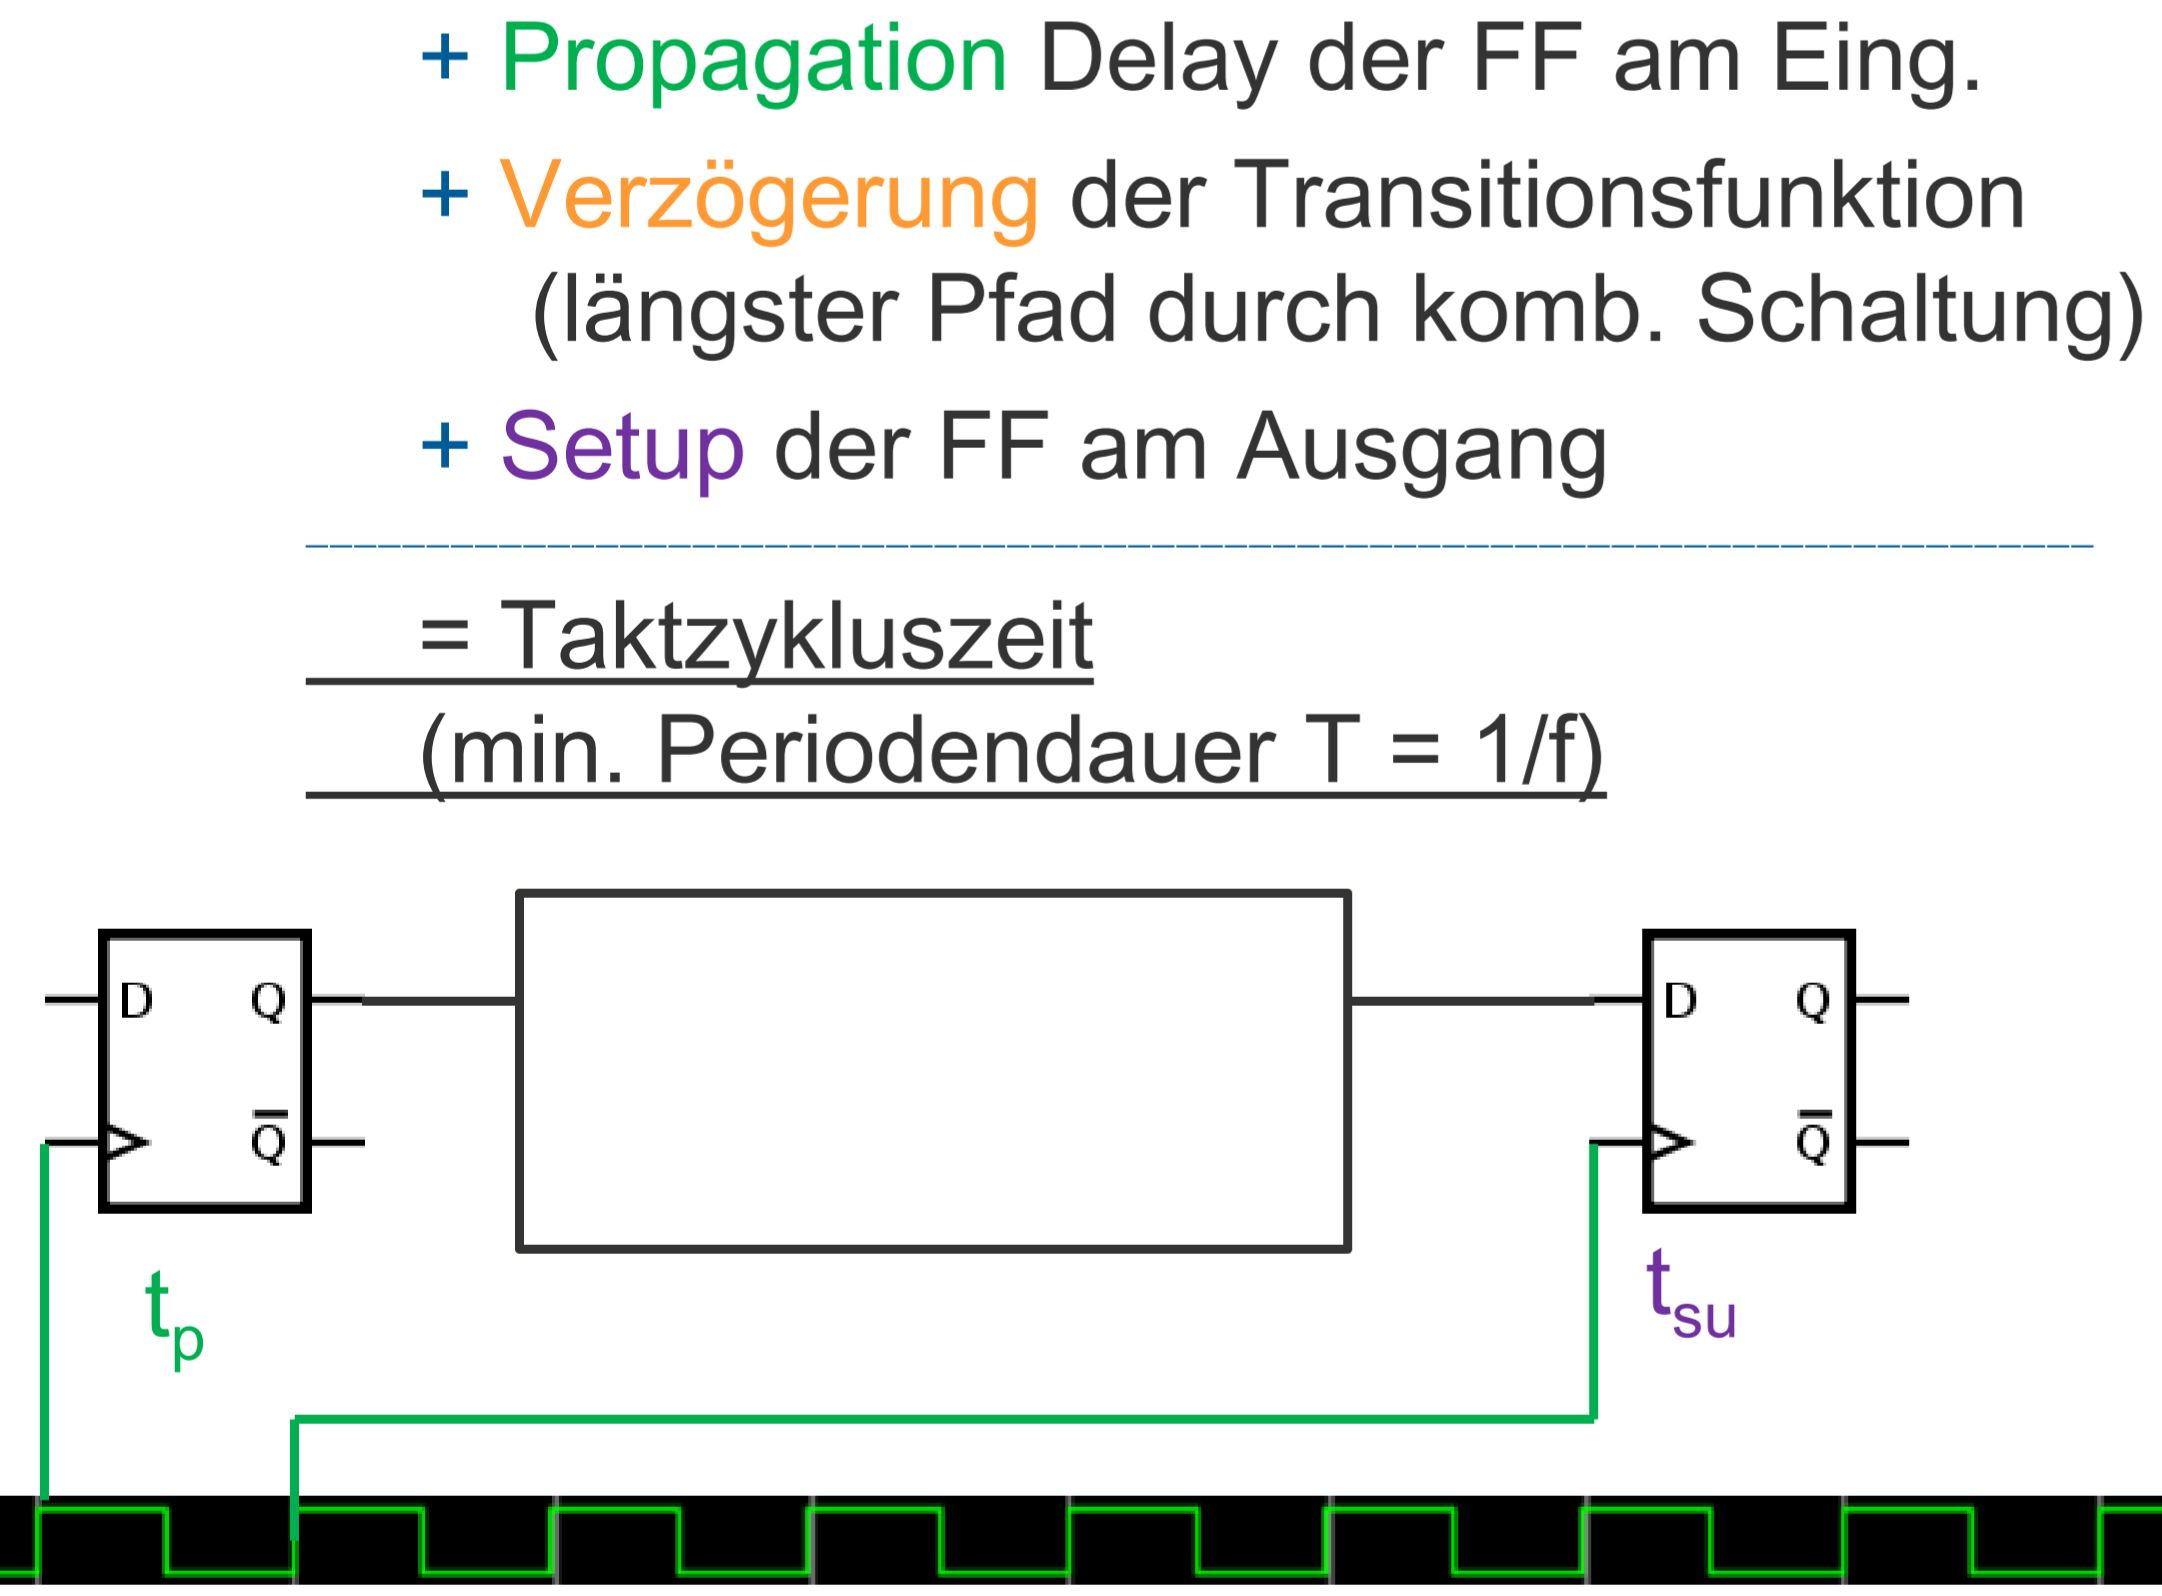
\includegraphics[width=0.5\columnwidth]{pics/laengster_pfad.jpg}
			\columnbreak
	\end{multicols}

\subsection{Flipflops und Latches}
	\subsubsection{Unterschied Flipflop und Latch}
%		\begin{minipage}{12 cm}
%			Taktzustandsgesteuerte Systeme haben den Nachteil, dass in ihrer transparenten Phase auch asynchrone Schaltvorg"ange stattfinden k"onnen. Echt synchrone Systeme "andern ihren Zustand nur bei der aktiven Flanke des Taktsignals. Genau in diesem Moment und sonst nie wird das Eingangssignal bei einem Speicherelement in den Speicher "ubertragen. Nur beim taktflankengesteuerten System wechseln die Ausg"ange immer genau zum Zeitpunkt der aktiven Taktflanke. Beim taktzustandsgesteuerten System sind w"ahrend der transparenten Phase auch Zustands"anderungen zwischen zwei Taktflanken m"oglich. \\
%			Taktflankengesteuerte Speicherelemente werden Flip-Flops genannt. Taktzustandsgesteuerte Speicherelemente werden Latches genannt
%		\end{minipage}
%		\begin{minipage}{0.5 cm}
%			\ 
%		\end{minipage}
%		\begin{minipage}{6 cm}
%			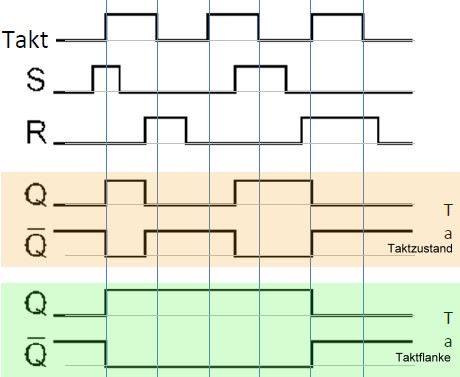
\includegraphics[width=0.9\textwidth]{pics/flipflop_latch}
%		\end{minipage}
		\begin{multicols}{3}
			\textbf{D-FF}\\
			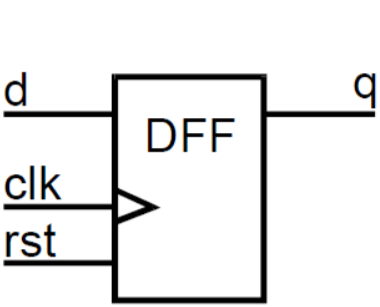
\includegraphics[width=0.2\columnwidth]{pics/d_flipflopO.png}
			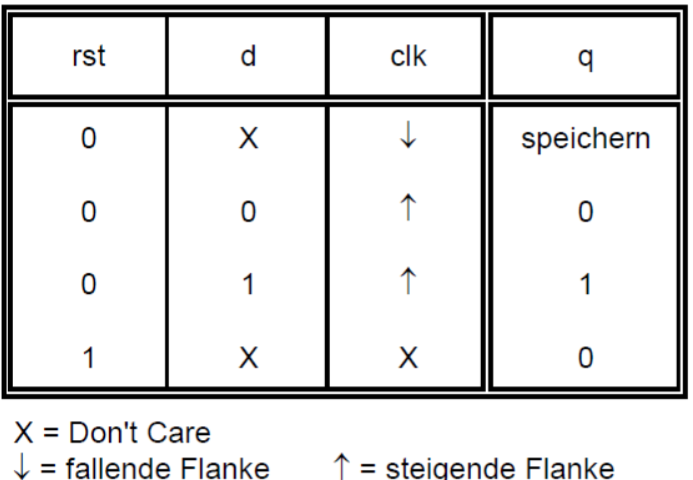
\includegraphics[width=0.78\columnwidth]{pics/d_flipflop.png}\\
			%Wechselt Zustand, nur bei (positiver Flanke des Taktsignals)
			\columnbreak
			
			\textbf{D-Latch}\\
			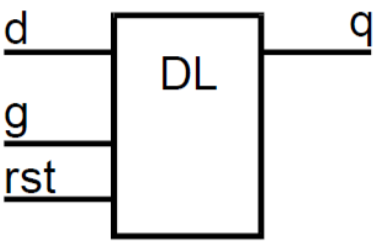
\includegraphics[width=0.2\columnwidth]{pics/d_latchO.png}
			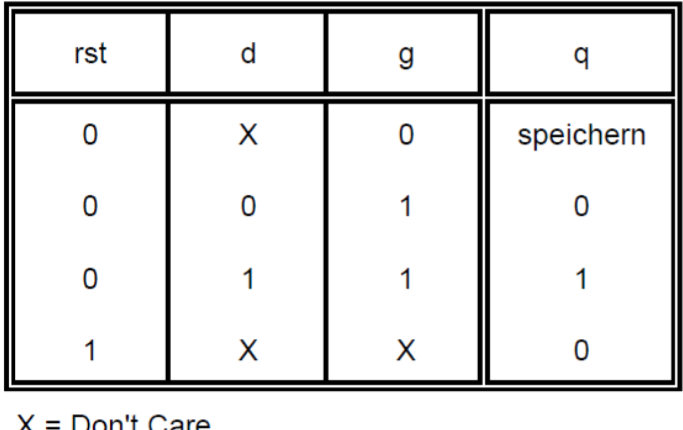
\includegraphics[width=0.78\columnwidth]{pics/d_latch.png}\\
			Wechselt Zustand, wann immer Level der Eingangssignale wechseln
			\columnbreak
			
			\textbf{Unterschied}\\
			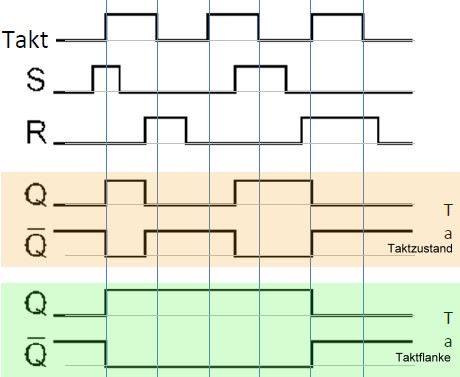
\includegraphics[width=0.8\columnwidth]{pics/flipflop_latch}
			\columnbreak
			
		\end{multicols}
			
		
	\subsubsection{Transmission Gate}
		\begin{minipage}{10 cm}
			Das Transmission Gate ist von seiner Funktion her ein einfacher Schalter, der Signale sowohl auf positivem, als auch auf negativem Pegel schalten kann.
		\end{minipage}
		\begin{minipage}{0.5 cm}
			\ 
		\end{minipage}
		\begin{minipage}{8 cm}
			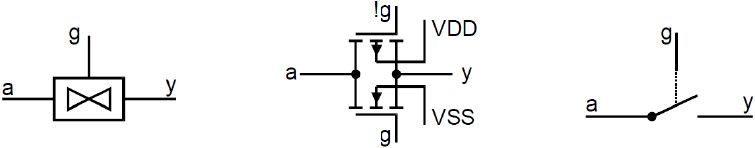
\includegraphics[width=0.9\textwidth]{pics/transmissiongate}
		\end{minipage}
		
	\begin{multicols}{2}
		\subsubsection{RS-Latch}
			\begin{minipage}{4 cm}
				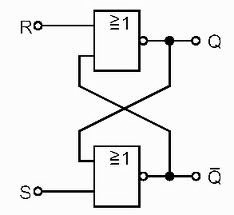
\includegraphics[width=0.9\textwidth]{pics/rs_latch}
			\end{minipage}
			\begin{minipage}{4 cm}
				\begin{tabular}{|cc|cc|}
					\hline
						S & R & $Q$ & $\overline{Q}$ \\
					\hline	
						0 & 0 & $Q$ & $\overline{Q}$ \\
						0 & 1 & 0 & 1 \\
						1 & 0 & 1 & 0 \\
						1 & 1 & \multicolumn{2}{c|}{nicht definiert} \\
					\hline
				\end{tabular}
			\end{minipage}
		
		\subsubsection{RS-Latch mit Clock}
			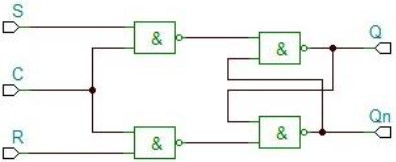
\includegraphics[width=0.4\textwidth]{pics/rs_latch_clock}
		\columnbreak
		
		\subsubsection{D-Latch}
			\begin{minipage}{4 cm}
				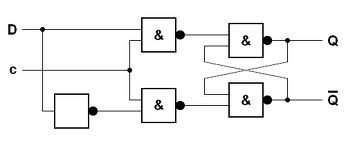
\includegraphics[width=0.9\textwidth]{pics/dlatch}
			\end{minipage}
			\begin{minipage}{4 cm}
				\begin{tabular}{|cc|cc|}
					\hline
						D & C & $Q$ & $\overline{Q}$ \\
					\hline	
						0 & 0 & $Q$ & $\overline{Q}$ \\
						0 & 1 & 0 & 1 \\
						1 & 0 & $Q$ & $\overline{Q}$ \\
						1 & 1 & 0 & 1 \\
					\hline
				\end{tabular}
			\end{minipage}
			
		\subsubsection{D-Flipflop mit Reset}
			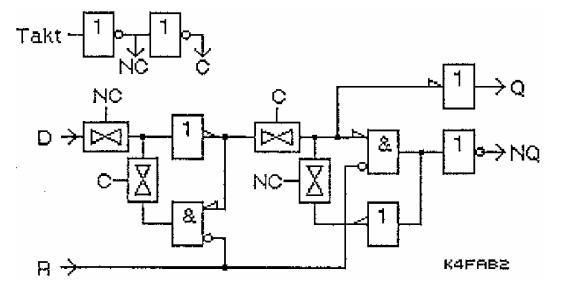
\includegraphics[width=0.4\textwidth]{pics/dflipflop}
	\end{multicols}
	
	\subsubsection{Setup- und Holdtime}
		\begin{minipage}{10 cm}
			\begin{compactitem}
				\item $t_s$= setup time $\rightarrow$ Minimale Zeitspanne, w"ahrend der ein Datensignal vor einer aktiven Clockflanke stabil sein muss, um zuverl"assig eingelesen zu werden.
				\item $t_H$= hold time $\rightarrow$ Minimale Zeitspanne, w"ahrend der ein Datensignal nach einer aktiven Clockflanke noch stabil bleiben muss, damit der Einlesevorgang des Datensignals erfolgreich abgeschlossen werden kann.
			\end{compactitem}
		\end{minipage}
		\begin{minipage}{0.5 cm}
			\ 
		\end{minipage}
		\begin{minipage}{8 cm}
			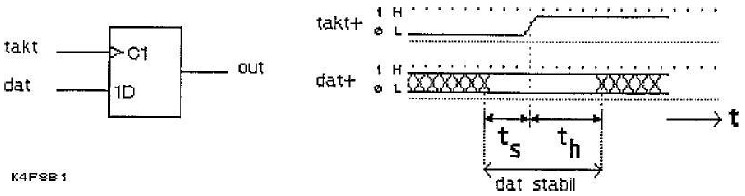
\includegraphics[width=0.9\textwidth]{pics/setupholdtime}
		\end{minipage}
	\newpage
		
\subsection{Beschreibung sequentieller Systeme}
	\begin{multicols}{2}
		\begin{compactitem}
			\item S: Menge der Zust"ande mit Zustandsaktionen
			\item I$\subseteq$S: Initalzust"ande
			\item T: Kombinatorische "Ubergangsrelation
			\item E: Eingangssignale
			\item A: Ausgangssignale
		\end{compactitem}
	\end{multicols}
	
	\begin{multicols}{2}
		\subsubsection{Tabellarische Beschreibung}
			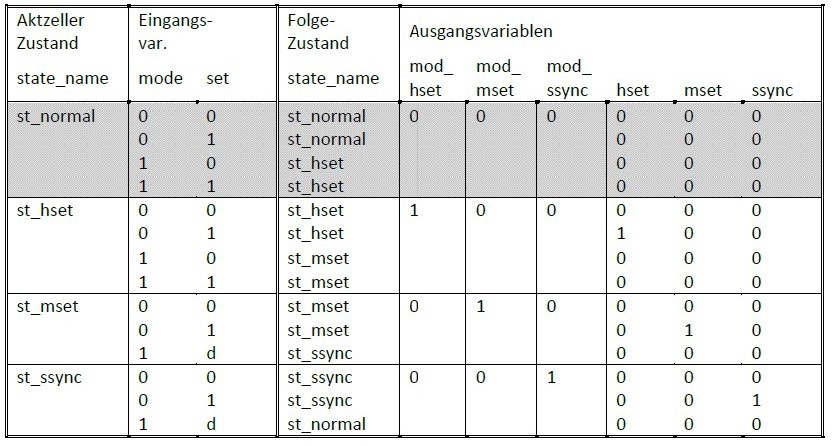
\includegraphics[width=0.49\textwidth]{pics/zustandstabelle}
		\columnbreak
		
		\subsubsection{Grafische Beschreibung (Zustandsdiagramm)}
			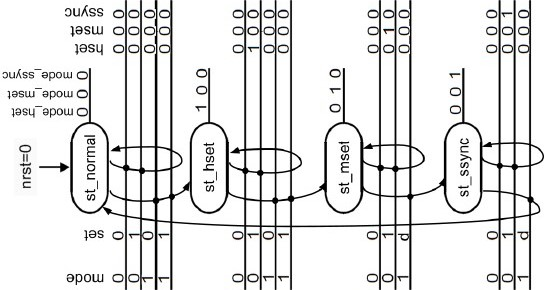
\includegraphics[width=0.5\textwidth]{pics/zustandsdiagramm}
	\end{multicols}
	Diese Beispiele visualisieren das sequentielle System des Watch-Controllers.
	
\subsection{Strukturen der Finite State Machine}
	\begin{multicols}{3}
		\subsubsection{Grundstruktur}
			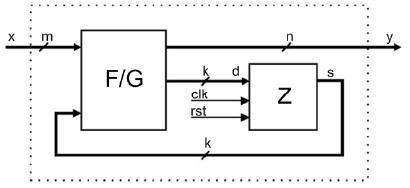
\includegraphics[width=0.3\textwidth]{pics/seq_grundstruktur}
		\columnbreak
		
			\begin{compactitem}
				\item s: Zustand, Zustandsvektor
				\item x: Prim"are Eing"ange, Eingangsvektor
				\item y: Prim"are Ausg"ange, Ausgangsvektor
				\item d: Speicheransteuerung, Folgezustand
				\item m: Anzahl Eing"ange
				\item n: Anzahl Ausg"ange
				\item k: Anzahl Speicherstellen
				\item F: Funktion f"ur die Ausg"ange
				\item G: Funktion f"ur die Speicheransteuerung
				\item Z: Zustandsspeicher
				\item I: Index der aktuellen Taktflanke (Taktflankennummer)
			\end{compactitem}
	\end{multicols}
	
	\begin{multicols}{3}
		\subsubsection{Mealy-System}
			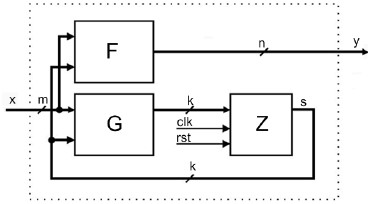
\includegraphics[width=0.26\textwidth]{pics/seq_mealy}
			Ausg"ange h"angen vom momentanen Zustand und den aktuellen Eing"angen ab.
			\columnbreak
			
		\subsubsection{Moore-System}
			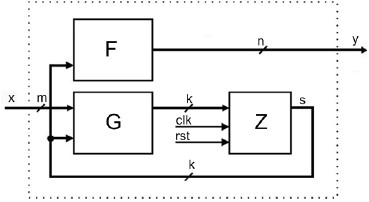
\includegraphics[width=0.26\textwidth]{pics/seq_moore}
			Ausg"ange h"angen nur vom momentanen Zustand ab und "andern mit der Clock Flanke.
			\columnbreak
			
		\subsubsection{Medwedjew-System}
			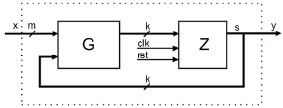
\includegraphics[width=0.3\textwidth]{pics/seq_medmedjew}
			Die prim"aren Ausg"ange entsprechen dem Zustandsvektor.
			\columnbreak
	\end{multicols}
	
\subsection{Zustandscodierung (ZC)}
	k: Anzahl Speicherstellen (1 Bit ist eine Speicherstelle), p: Anzahl Zust"ande
	\begin{multicols}{3}
		\begin{compactitem}
			\item Bin"ar: Alle Zust"ande werden der Reihe nach durchnummeriert. \\
			$k = \lceil \frac{log_{10}(p)}{log_{10}(2)} \rceil = \lceil log_2(p)\rceil, \; p < 2^k $
			Anz. m"ogl. ZC: $q = (2^k!)/(2^k - p)!$
			\item ONE-HOT: Nur eine Speicherstelle im Code hat jeweils den Wert 1. Alle anderen besitzen den Wert 0 (z.B. 001, 010, 100)
			\item ONE-COLD: Nur eine Speicherstelle im Code hat jeweils den Wert 0. Alle anderen besitzen den Wert 1 (z.B. 110, 101, 011)
		\end{compactitem}
	\end{multicols}

%\subsection{Synthese von Zustandsmaschinen}
%	\begin{multicols}{2}
%		\begin{enumerate}
%			\setlength{\itemsep}{1pt}
%			\setlength{\parskip}{0pt}
%			\setlength{\parsep}{0pt}
%			\item Zustandsdiagramm aufstellen
%			\item Zustandskodierung zuweisen
%			\item Zustandstabelle nach festen Regeln aufstellen
%			\item Speicheransteuer-Funktionen bestimmen
%			\item Ausgangs-Funktionen bestimmen
%		\end{enumerate}
%	\end{multicols}